%%==================================================
%% chapter03.tex for SJTU Master Thesis
%% Encoding: UTF-8
%%==================================================

%%%%%%%%%%%%%%%%%%%%%%%%%%%%%%%%%%%%%%%%%%%%%%%%%%%%%
%%
%%   同义词对称可搜索加密
%%
%%%%%%%%%%%%%%%%%%%%%%%%%%%%%%%%%%%%%%%%%%%%%%%%%%%%%
\chapter{同义词对称可搜索加密}
\label{chap:synonym}

到目前为止,对称可搜索加密技术已得到广泛的研究,各种复杂的条件搜索加密技术也被深入的研究并取得了实质性的成果。然而在复杂的多变的云计算环境下,我们需要研究的知识点范畴广和面对的用户群里基数大。为此,我们不得不进一步挖掘出一些尚未提出并具有实际意义的问题。在前人的工作指导下,本文解决了相似搜索的另一个场景 --- 同义词搜索。

在本章,我们提出了一个支持同义词搜索并具有强安全性的对称可搜索加密方案。为此,我们首先定义了方案的系统模型和攻击模型;然后定义其算法框架;针对方案框架的各个算法,逐个给出它们的详细实现细节;最后我们对该方案进行了严格的安全性证明和性能分析。



%%%%%%%%%%%%%%%%%%%%%%%%%%%%%%%%%%%%%%%%%%%%%%%%%%%%%
%%
%%   方案模型
%%
%%%%%%%%%%%%%%%%%%%%%%%%%%%%%%%%%%%%%%%%%%%%%%%%%%%%%
\section{方案模型}
\label{sec:synonym_model}

在该小节,我们从已有的方案中抽象出将研究的问题;然后针对我们的问题,提出了相应的系统模型和有效的攻击模型;为了实现方案的详细细节,我们引入一些相关的符号及其描述,同时定义了方案的信息泄漏;最后,我们简略地描述了方案的基本框架。

%%在该小节,我们从已有的方案中抽象出将研究的问题;然后针对我们的问题,提出了相应的系统模型;并针对该系统模型,我们提出了有效的攻击模型;为了实现方案的详细细节,我们引入一些相关的符号及其描述,同时定义了我们方案中的信息泄漏;最后,我们简略地描述了我们方案的基本框架。

\subsection{问题提出}
\label{sec:synonym_problem}

%生活在网络高速发达的时代,数据的产量以指数的量级增长,大数据的时代已到来,为解决人们难以应付的难题,可搜索加密方案被提出并解决了大数据中存储和计算的问题。然而,在网络竞争时代,

可搜索加密技术解决了外包数据的安全和高效搜索的难题。然而,在互联网快速发展的时代下,人们在工作中的强度日益增加,致使人们的记忆力也随着超载工作量的过度消耗而呈现下降趋势。由于人们记忆能力的周期的缩短和人员频繁的变换,使得一段时间之后,他们对之前使用过的文档及其内容的记忆已模糊不清甚至完全遗忘。此情景的一个典型的示例如图\ref{fig:synonym_problem}所示。首先,使用云计算平台服务的数据所有者将文档外包至不可信的云端;一段时间后,数据所有者想要查找包含“文件”含义的关键字的文档时,其可能因忘记不知道文档中到底包含“paper” 还是“document”?为此,用户不得不逐个尝试所有具有该含义的单词,直至找到所需的答案为止。在按计算收费的时代,这显然是不合理的,同时也增加了网络带宽和用户的响应时间。%为解决此场景引出的问题,该章提出了一个新的解决方案 --- 同义词对称可搜索加密技术。
\begin{figure}[!htp]
 \centering
 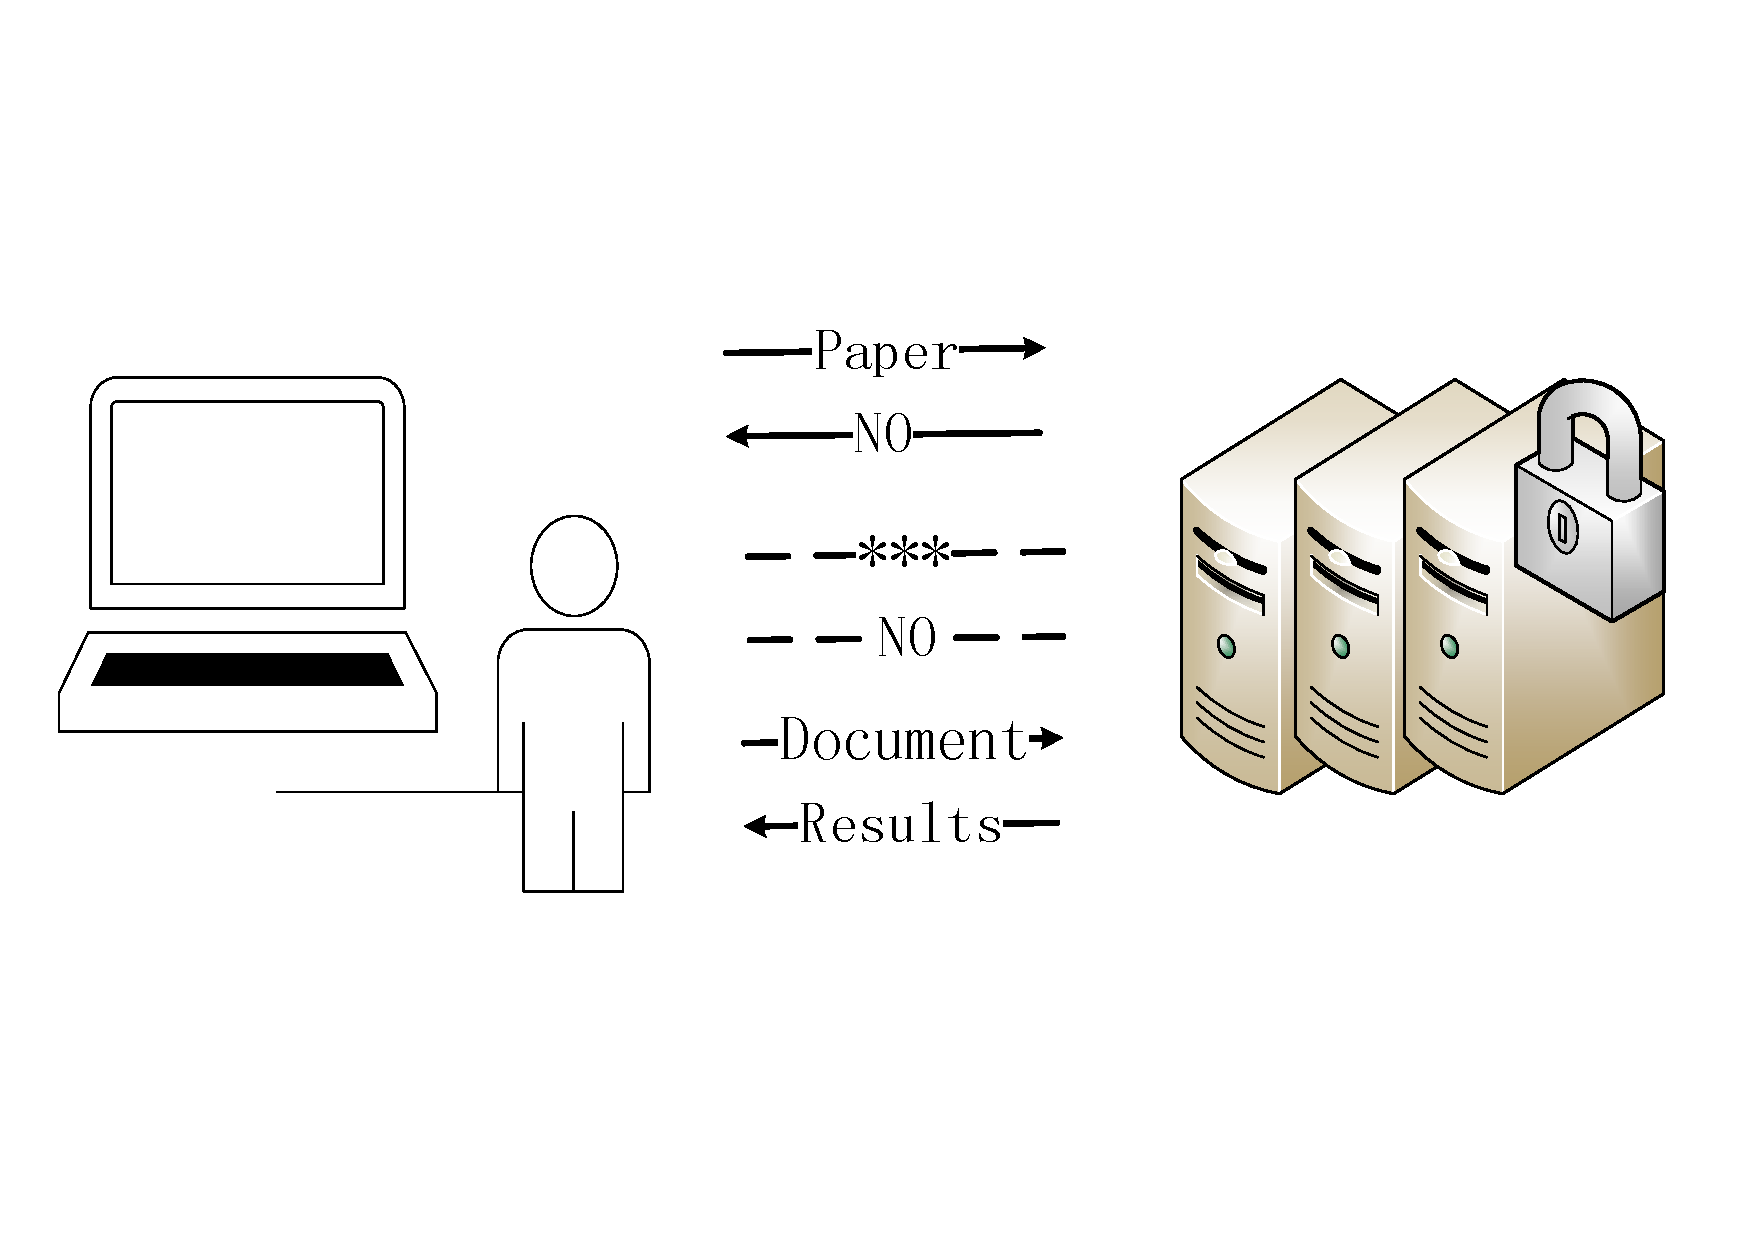
\includegraphics[angle=0,origin=br,width=15cm]{chap4/problem.pdf}
 \bicaption[fig:synonym_problem]{同义词可搜索加密方案的示例}{同义词可搜索加密方案的示例}{Fig}{An Example of the Synonym Search}
\end{figure}



\subsection{系统模型}
\label{sec:synonym_model_system_model}

在我们的方案中,支持同义词搜索的系统模型(如下图\ref{fig:synonym_system_model}所示)包括三部分 --- 数据所有者(Owner),授权用户(Users)和云服务提供商(Provider)。这三部分在系统中分别承担不同的角色。数据拥有者是数据的源头和拥有系统的抉择权,授权用户是系统中最频繁的访问者,而云服务提供商是系统的服务提供者和数据的响应者。
\begin{figure}[!htp]
 \centering
 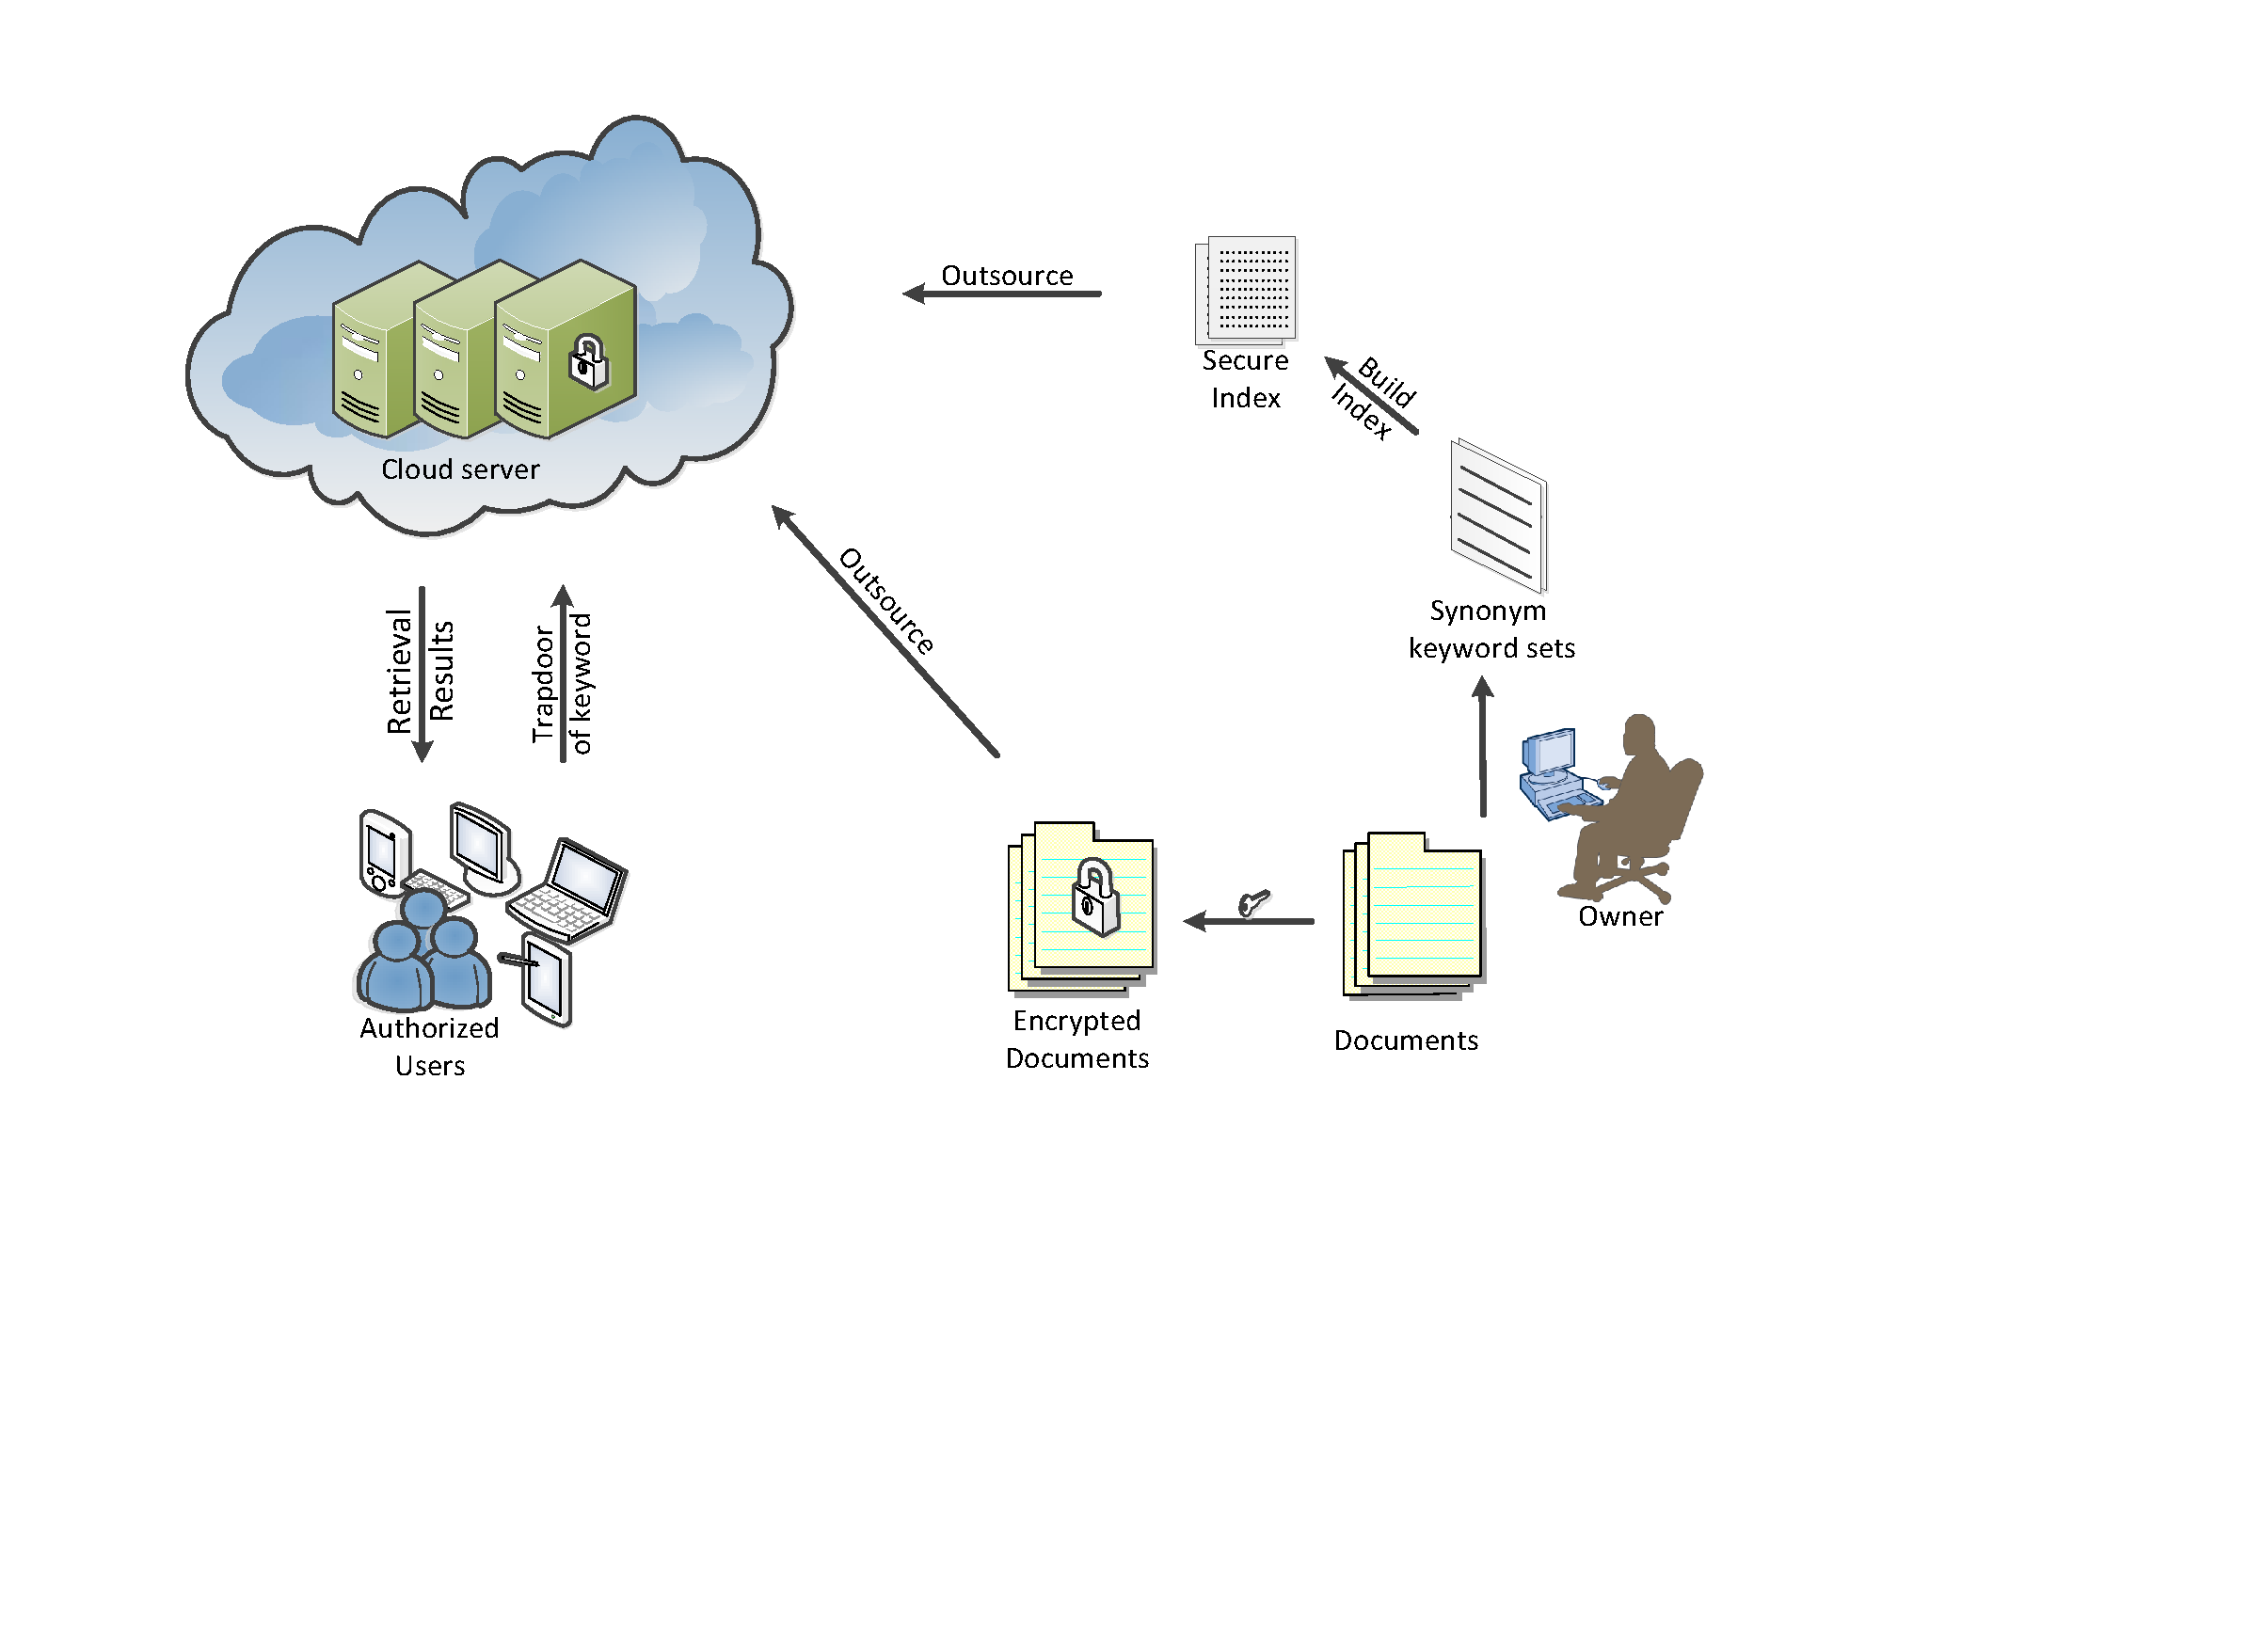
\includegraphics[angle=0,origin=br,width=15cm]{chap4/system_model.pdf}
 \bicaption[fig:synonym_system_model]{同义词可搜索加密系统模型}{同义词可搜索加密系统模型}{Fig}{The System Model of Synonym Search}
\end{figure}


\begin{enumerate}
  \item
  \textbf{数据所有者:} 数据所有者是系统的主体,拥有系统中最核心的部分---数据。数据拥有者往往由一个公司、组织或团体组成。同时,数据拥有者需要考虑系统的性能、功能和其它各种因素。一般情况下,当数据拥有者想利用外包端的便利服务时,需先购买云服务,将所有的数据首先加密,然后存储到云服务提供商。



  \item
  \textbf{用户:} 用户是系统的使用者,往往是系统中最大的人群(包括数据所有者)。用户往往不考虑系统的任何细节,只希望利用系统提供的便利和安全性。通常情况下,如果一个用户想要使用系统的查询功能,首先他必须征求数据拥有者的允许---即获得请求数据的安全密钥,成为合法的请求者;然后利用安全密钥生成单词陷门,并提交任务给云端;最后,在收到响应结果后,对其进行解密,获得所需的文档。在我们系统中,返回的结果包括所有包括该单词和与它有相同含义的单词的文档。



  \item
  \textbf{云服务提供商:} 云服务提供商是系统的客体 --- 系统功能服务者,用于对外包数据进行存储和计算,是系统必不可少的一部分。通常情况下,首先接收数据所有者提交至云端的加密数据和索引,并提供对数据的计算和备份工作。当收到用户提交的查询请求时,然后利用强大的计算能力对数据进行查询操作,并将匹配的结果返回给请求者,若不存在则返回空。
\end{enumerate}

在同义词可搜索加密方案中,云服务提供商返回的结果集包括两部分:(1)包含待查单词的文档;(2)包含与待查单词有相同含义的单词的文档。即返回的信息可描述为:$ED = \{ ED_i | w \in D_i, w \in S_w \}$。并且证明我们方案具有non-adaptive安全。

%%在我们的系统中,若云服务提供商是安全并且诚实的,因而我们系统中外包的数据是安全的 --- 数据使用安全函数加密。但是,在通常情况下,云服务提供商虽然表面上遵照系统协定提供安全的云服务,而本身又是“honest-but-curious” ---- 因对数据好奇而暗地里偷偷地分析用户查询的数据,然后根据其他知识(例如单词的统计信息)来推断用户所搜索的真实单词,这足以说明我们方案仍存在一定的信息泄漏。为此,我们必须精确量化出系统信息泄漏的大小,通常将云服务器视为具有最强计算能力的敌手,能分析出的数据即为系统的信息泄漏量。

\subsection{攻击模型}
\label{sec:synonym_model_attack_model}

在我们的系统中,若云服务提供商是安全并且诚实的,因而我们系统中外包的数据是安全的 --- 仅使用了安全的伪随机函数和$SKE.Enc$对数据加密。不幸的是,通常来说云服务提供商是“honest-but-curious” --- 即遵照系统所定义的协定进行操作,同时因对数据好奇而暗地里偷偷地分析用户查询的数据,然后根据一些其他知识(例如单词的统计信息)来推断用户所搜索的真实单词,这足以说明以上方案仍存在一定的信息泄漏。为此,我们必须精确地量化出系统信息泄漏的大小,通常将云服务器视为具有最强计算能力的敌手,能分析出的数据即为系统的信息泄漏量。为了衡量我们所定义信息泄漏的正确性,引入了安全的分析模型,以证明方案除了泄漏必不可少的信息之外,不泄露其他任何的信息。为了证明方案具备Non-adaptive安全,假设$\mathcal{A}$ 是多项式的敌手,$\mathcal{S}$是模拟者,方案的攻击模型如下:


%%在我们的方案中,如果云服务提供商是绝对安全并且诚实的,则我们系统中外包的数据必是安全的 --- 仅使用伪随机函数和$SKE.Enc$对数据加密。不幸的是,通常来说云服务提供商是“honest-but-curious” --- 即遵照系统所定义的协定进行操作,同时因对数据好奇而暗地里偷偷地分析用户查询的数据,然后根据一些其他知识(例如统计信息)来推断我们查询的内容,这致使我们的数据仍处理一定的风险。为此,我们必须清楚地了解到云服务到底能分析出多少信息。为了分析我们系统泄漏信息量的大小,我们通常将云服务作为敌手,在他们有最强的计算能力的亲情况下,分析出的数据即为我们系统的信息泄漏量。为了衡量我们所定义信息泄漏的正确性,引入了安全的分析模型,以证明方案除了泄漏我们所定义的信息之外,不泄露其他任何的信息。这里我们定义我们方案具有Non-adaptive安全,假设$\mathcal{A}$是多项式的敌手,$\mathcal{S}$是模拟者,方案的攻击模型如下:

\begin{center}
\begin{tabular}{ l l }
    $\textbf{Real}_{SSE,\mathcal{A}}(k)$  &  $\textbf{Sim}_{SSE,\mathcal{A},\mathcal{S}}$    \\
    \quad $K \leftarrow SSGen(1^k)$ & \quad $(H,st_\mathcal{A}) \leftarrow \mathcal{A}(1^k)$ \\
    \quad $(st_\mathcal{A},H) \leftarrow \mathcal{A}(1^k)$ &\quad $V^* \leftarrow S(\tau (H))$\\
    \quad parse $H$ as $(D,w)$          &   \quad output $V^*$ and $st_\mathcal{A}$     \\
    \quad $(SI,KED) \leftarrow SSEnc(D,K,SD)$            &   \\
    \quad for $1 \leq i \leq q $                 &   \\
    \quad \quad $T_{w_i} \leftarrow SSTrapdoor(w_i,K)$    &   \\
    \quad let $T_w = (T_{w_i}, ..., T_{w_q})$              &    \\
    \quad output $V = (SI,KED,T_w)$ and $st_\mathcal{A}$    &
\end{tabular}
\end{center}



\subsection{相关定义}
\label{sec:synonym_model_related_definition}

%%在这里,我们定义了一些与方案相关的符号,如下(Note:X --- 代表是一个数据结构,包括链表、数组或文档等等;n --- 任意大小):
\begin{itemize}
%  \item
%  $|X|$ --- 结构X的长度,即X中单词的个数。

  \item
  $ [n] $ --- 表示$n$个元素的集合,等价于 $\{ 1, ..., n \}$。

  %\item
%  {$ max(|S|) $} --- 如果S是集合,则它代表集合S的元素数目|S|;若S是集合的集合,则它表示集合S 中所有元素的最大数目,即$max\{|S_i|$ | $S_i \in S\}$。

  \item
  $D$ --- 所有待外包的文档的集合,$n$个文档的集合 $D$ = ($ D_1, D_2, ..., D_n $)。

  \item
  $ID(D)$ --- 文档$D$的ID信息,可以用数字表示也哈希值来唯一表示。

  \item
  $ED$ --- 加密文档的结合,$n$个密文文档的集合 $ED$ = ($ ED_1, ED_2, ..., ED_n $)。

  \item
  $KED$ --- 所有加密文档键值对$<$ $ID(D_i)$, $ED_i$ $>$的集合($ ED_i \in ED $)。

  \item
  $W(X)$ --- 结构$X$中所有不同单词所组成的集合,表示为:$W(X) = (w_1, w_2, ..., w_{|W(X)|})$。

  \item
  $D_w,SD_w$ --- $D_w$是仅包括单词$w$的所有文档的集合;$SD_w$是包括单词$w$和其同义词的文档的集合。

  \item
  {$SD$}--- 同义词字典的集合,它必须包含集合$W(D)$中的所有单词。根据所定义环境的不同,集合中元素也不相同。$m$个元素的集合$SD$,表示为:$SD$ = ($ w_1, ..., w_m $)。

  \item
  $ S_w $ --- 单词$w$的所有同义词的集合,描述为:$ S_w = (w_1, w_2, ..., w_{|S_w|}) $。

   \item
  $ SID_w $ --- 包含单词$w$的文档的ID集合,定义$ SID_w = \{ID(D_i) $ $|$ $ w \in D_i\}$, $SID$ = $\{SID_w$ | $w_i \in W(D) \} $。

  \item
  ${SI}$ --- 安全索引结构,由数据拥有者生成,并存储在云服务端。在我们系统中使用数组和查询表来维护。

  \item
  $ T_w $ --- 单词$w$的陷门信息。它使用伪随机函数生成,用于在搜索过程中作文查询口令。

  \item
  $ ESD_w $ --- 用户在查询后,由服务器返回的加密的文件集合。


%%  \item
%%  $F(K,*)$ --- 如果我们定义函数$F$为: $ \{0, 1\}^k * \{0,1\}^n \rightarrow \{0, 1\}^m $,且在多项式时间内,函数F是可计算的和对于一个具有多项式访问oracle的敌手A,有: $|Pr[A^{f_k(.)} = 1 : K \leftarrow \{0,1\}] - Pr[A^{g(.)} = 1: g \leftarrow Func[n,m]]| \leq negl(k)$,则称函数F 为伪随机函数(PRF),若函数F是双射,我们称它为伪随机置换(PRP)。
%%
%%  \item
%%  ${ SKE = (Gen, Enc, Dec) }$ --- 定义SKE是私钥加密方案。在标准SKE中,Gen是伪随机函数, 用于生成密钥K;Enc用于将给定的值进行加密;而Dec则用于解密。对于任意给定的两个密文,我们不能判断是否被同一个密钥加密。
\end{itemize}

%
% Definition: Synonym Function
%
\textbf{同义词函数(Synonym Function)} 对于任意给定的两个单词$w_1$和$w_2$,定义:
\begin{equation}
SF(w_1, w_2) =
\begin{cases}
1 & \text{ if ${w_1}$ and ${w_2}$ is synonym}
\\
0 & \text{ otherwise }
\end{cases}
\end{equation}
在上述公式中,如果输出结果为1,则称单词$w_1$和$w_2$相似,称函数$SF$为相似判断函数(简称相似函数)。

%
% Synonym dictionary
%
%%\textbf{同义词集合(Synonym Sets)} 对于给定的单词w ($ w \in SW$),定义同义词集合为:$ SWS = \{S_{w_i}$ $|$ $ w_i\in S_w \} $。在我们的系统中对于$SW$,我们取英文字典中的所有单词,其原因是:如仅包含单词W(D),若我们查询单词“document”时,而文中不包括“document”仅包含“paper”,则输入则无效,这将大大降低方案的可用性。在实际中,我们可以根据环境的不同来定义SW,甚至我们能动态地根据环境信息搜索建立SW集合。



%
% Definition: Information Leakage
%
\textbf{信息泄漏} 在我们的方案中,我们主要分析我们所定义场景下的信息泄漏情况,我们定义该方案信息泄漏包括文档大小、访问模式和搜索模式。这里我们不考虑文档大小,仅从搜索模式和访问模式信息泄露进行分析。

\textbf{查询历史:} 具体定义请参见\ref{defn:attack_history}。

\textbf{搜索模式:} 给定文档集$D$和$q$次查询历史$H$,定义搜索模式如下:\\
 $\sigma(H) = \begin{bmatrix}
 &x_{1,1}  &x_{1,2}  &...  &x_{1,q} \\
 &x_{2,1}  &x_{2,2}  &...  &x_{2,q} \\
 & . & .   &...      &. \\
 & . & .   &...      &. \\
 & . & .   &...      &. \\
 &x_{q,1}  &x_{q,2}  &...  &x_{q,q} \\
\end{bmatrix}$,其中$x_{i,j}$可能取值0、1、2。若$x_{i,j}$为0 --- 表示$w_i$和$w_j$为不相等且没有相同的同义词集合$S_w$;取值1 --- 表示$w_i$和$w_j$不相等但是有相同的同义字集合;取值2 --- 表示$w_i$ 和$w_j$ 为相同的单词。

\textbf{访问模式:} 对于给定文档集$D$和$q$次查询历史$H$,定义访问模式 $\partial(H) = (SD(w_1), SD(w_2), ... SD(_q))$,$SD(w_i)$ = $\{D(w_j)$ | $w_j \in S_w$ $\}$。

\textbf{Trace:} 对于给定大小为$n$的文档集$D$和$q$次查询历史$H$,定义其Trace信息为元组:$\tau(H) = (|D_1|, ..., |D_n|, \sigma(H), \partial(H))$。


\subsection{方案描述}
\label{sec:synonym_model_scheme_description}
%在我们的方案中,主要解决对称可搜索加密环境下同义词搜索(SSSE)的场景,即输入单词w,即返回包含单词w 的文档,同时返回包括和单词w有相同函数的文档的问题。下面简单描述我们的方案。\\

下面我们简单地描述我们方案:\\
%
% Definition: Synonym Searchable Encryption
%
\textbf{Synonym Searchable Encryption(SSSE):} 方案包括由5个基本的算法组成,定义:$SSSE$ =($SSKeyGen, SSEnc, SSTrapdoor, SSSearch, SSDec$)。
\begin{description}
  \item[$\{K\} \leftarrow SSKeyGen(1^k)$:]是一个概率密钥生成算法,输入安全参数$k$和输出密钥$K$。
  \item[$\{SI, KED\} \leftarrow SSEnc(D, K)$:]是方案中主要的加密模块,输入参数文档集合$D$和密钥$K$,输出安全索引$SI$和加密文档$KED$。主要包括文档加密函数($SSDEnc$)和安全索引建立函数($SSBuildSI$)。
  \item[$\{T_w\} \leftarrow SSTrapdoor(w, K)$:]是一个确定性的算法(可能是概率算法)。对于一个给定的单词$w$,在密钥$K$下,生成陷门${T_w}$。
  \item[$\{ESD_w\} \leftarrow SSSearch(T_w, SI, KED)$:]是一个确定性算法。输入待查询单词$w$的陷门$T_w$、$SI$ 和$KED$,查询并输出同义词结果集${ESD_w}$。
  \item[$\{PSD_w\} \leftarrow SSDec(ESD_w, K)$:]是一个确定性的算法,用于解密。使用返回的结果集${ESD_w}$和加密密钥$K$,并输出解密的文档${PSD_w}$。
\end{description}


%%%%%%%%%%%%%%%%%%%%%%%%%%%%%%%%%%%%%%%%%%%%%%%%%%%%%
%%
%%   算法框架与方案细节
%%
%%%%%%%%%%%%%%%%%%%%%%%%%%%%%%%%%%%%%%%%%%%%%%%%%%%%%
\section{算法框架及细节}
\label{sec:synonym_scheme}

在描述我们的方案之前,仅仅考虑一个简单的情况 --- $SD$中每个单词仅存在一个含义。基于这样的假设,我们设计了一个支持同义词搜索的解决方案并描述方案中各算法的详细实现流程。然后我们阐述了如何将我们方案应用于一词多义的情形并分析我们方案的优势。在详细描述我们方案之前,我们重新回顾同义词字典和同义词集合的概念。

\textbf{关于$SD$的扩展:} 为了使该方案更具通用性,方案中定义同义词字典$SD$为按字典排序的所有的单词集合。它不仅包括$W(D)$中的所有单词,而且包含与文档中单词有相同含义的所有单词。考虑此情况的原因在于:如果我们外包有单词“Paper”但不包含单词“Document”的文档集合$D$至远程服务器;一段时间后,授权用户键入单词“Document”去查找,由于键入没有命中,服务器不得不返回无效的结果集。此时,用户不得不逐个地尝试所有具有相同含义的单词,找到所要查询的文档未知。这将大大降低方案的灵活性和可通用性。另外,用户通常希望在不同的环境下有不同的同义词集合,通常我们可能根据某领域内用户的查找知识来动态建立同义词字典。例如,在医疗行业,同义词字典的集合与其它领域可能有所不同,我们可以根据客户的要求来建立$SD$。 这样定制的同义词集合将使我们方案的查询性能更好和返回的结果集更有意义。

\textbf{同义词集合的构建:}通常情况下,同义词集合仅仅考虑文档中所有不同单词集合$W(D)$,而忽略了其它单词。在我们构建的方案中,基于同义词字典,建立同义词集合如下:
\begin{enumerate}
  \item
  对每个单词$w \in W(D)$,初始化单词的同义词集合$S_w = \{w\}$;
  \item
  然后对每个单词 $w_i \in \{SD \setminus w\}$,计算$SF(w, w_i)$,如果结果为1,则插入单词$w_i$ 至集合$S_w$,否则跳过它;
  \item
  最后定义文档的同义词集合$SWS = \{S_w | w \in W(D) \}$。
\end{enumerate}



\subsection{\textbf{框架详细描述}}
\label{sec:synonym_scheme_description}

\textbf{同义词对称可搜索加密:} 定义同义词对称可搜索加密方案由五个算法组成即 $PSSSE = (SSKeyGen, SSEnc, SSTrapdoor, SSSearch, SSDec)$。$SSKeyGen$用于生成密钥;$SSEnc$算法由三个子算法($SSInitSets$ --- 用于初始化文档集合,$SSDEnc$ --- 加密文档,$SSBuildSI$ --- 对文档建立安全索引)组成;$SSTrapdoor$ 生成单词的陷门;$SSSearch$通过陷门查找结果集;$SSDec$仅仅是个简单的解密过程。


%%%In the detailed algorithms definition, we will make full use of the functions $F$, $G$, $P$, $\mathcal{H}$, $\mathcal{G}$, where $F$, $G$ and $P$ are pseudo-random function, $\mathcal{H}$ is the pseudo-random permutation, and $\mathcal{G}$ is pseudo-random generator. To the store the secure index, we use search table $A_t$ and array $A_s$ where $A_t$ is search table of keyword trapdoor in secure index, and $A_s$ is array including all nodes of document ID in $SI$. We define: $SIZE(A_t)$ and $SIZE(A_s)$ are the size of padding additional entries, $max(|SID|)$ and $max(|SWS|)$ are respectively the maximum size of any one element in $SID$ and $SWS$, e.g. $max(|SID|) = (|SID_w|$  $|$  $SID_w \in SID$), where $|SID_{w_i}| \leq |SID_w|$ for any $w_i \in W(D), SID_{w_i} \in SID $. A detailed description of our solution is in Figure \ref{fig:core_algorithm} (Note: in this solution, we only consider each keyword as one meaning, and we will introduce how to dispose of the context of multi-meanings of keyword in the subsequent subsection.)

在详细地描述我们的方案之前,这里首先定义一些将被使用的函数和数据结构,如下:
\begin{itemize}
  \item
  函数$F$、$G$和$P$是伪随机函数;

  \item
  $\mathcal{H}$是伪随机置换;

  \item
  $\mathcal{G}$是伪随机生成器;

  \item
  $A_t$是一个足够大的查询表,用于存储到此的陷门内容,通过此可以找到包含文档$ID$的信息。$SIZE(A_t)$ 表示查询表实际所使用的大小,即未填充时所使用的大小;

  \item
  $A_s$是一个足够大的数组,用户存储文档ID的内容,用户检索到加密文档。$SIZE(A_s)$表示存储文档$ID$ 实际所使用的空间大小。
\end{itemize}

PSSSE方案的各个算法具体实现如下:
%\fbox{
%  \parbox{1.0\textwidth} {
  %
  % insert a long text in here....
  %
    \begin{enumerate}
      %
      % 1. SSKeyGen
      %
      \item
      \textbf{$ \{ K \} \leftarrow SSKeyGen(1^{k}): $} \\
       该算法从集合$ {\{0,1\}}^{k} $中随机选取密钥${ K_1, K_2, K_3 }$,并且调用$SKE.Gen$生成${ SK \leftarrow SKE.Gen(1^{k}) }$,输出$K$ = ($K_1$, $K_2$, $K_3$, $SK$)。

      %
      % 2. SSEnc
      %
      \item
      \textbf{$\{ SI, KED \} \leftarrow SSEnc(D, K):$ } \\
      该算法包括三个子算法$(SSInitSets, SSDEnc, SSBuildSI)$。$SSInitSets$用户初始化操作,$SSDEnc$用于加密文档,$SSBuildSI$用于建立安全索引。它们按如下的顺序执行($SD$在前面被建立):

      \begin{enumerate}
      %
      % SSInitSets
      %
      \item
      \textbf{$ (SWS, SID) \leftarrow SSInitSets(D, SD). $}

      \begin{itemize}
        \item ${ W(D) \leftarrow D }$,遍历文档集$D$,提取出所有不同的单词组成集合:$W(D) = \{w_1, ..., w_{|W(D)|} \}$。

        \item 对每一个单词$ w \in W(D) $,浏览文档$D$构建包含单词$w$的文档的ID集合:$SID_w = \{ID(D_i)$ $|$ $w \in D_i \})$,定义: $SID = \{ SID_{w}$ $|$ $w \in W(D) \}$, 并且确保每个集合的大小与最大集合大小相等。若小于最大集合则使用随机生成的唯一的字符串填充。

        \item 对每个单词$w \in W(D)$,按照上述同义词集合构建过程构建文档的同义词集合。如何集合大小不相等,则通过填入随机的值使得每个集合的大小相等,生成新的集合$SWS$。

      \end{itemize}

      %
      % SSDEnc
      %
      \item
      $ (KED) \leftarrow SSDEnc(SK, D). $ \\
      对每个文档$D_i \in D$,加密生成$ED_i \leftarrow SKE.Enc(SK, D_i)$。然后对每个$ED_i$,设置:$KED_i = <ID(D_i), ED_i>$,并定义$KED = \{ KED_i | i \in [|D|]\}$。

      %
      % SSBuildSI
      %
      \item
      ${ (SI) \leftarrow SSBuildSI(K, SWS, SID). }$ \\
      该算法用于建立方案的核心检索结构 --- 安全索引$SI$,加速查找过程。详细实现细节,请参考算法 \ref{alg:SSBuildSI}。
      % \ref{alg:SSBuildSI}
      \end{enumerate}
      最后,将安全索引$SI$和加密文档内容$KED$外包到远程服务器。


      %
      % 3. SSTrapdoor
      %
      \item
      \textbf{ $ \{ T_w \} \leftarrow SSTrapdoor(w, K): $ }\\
      授权用户使用陷门生成函数输出单词$w$的陷门内容如下:$ T_w =$ $($ $F_{K_1}(w)$, $G_{K_2}(w)$, $P_{K_3}(w)$ $)$,并将请求送至服务器。


      %
      % 4. SSSearch
      %
      \item
      \textbf{$ \{ ESD_w \} \leftarrow SSSearch(T_w, SI, ED): $} \\
      一旦服务器收到远程请求者的陷门,便开始查找安全索引和加密文档,并返回匹配的答案给请求者。具体的实现过程在算法\ref{alg:SSSearchESR}中描述。


      %
      % 5. SSDec
      %
      \item
      \textbf{${ \{PSD_w\} \leftarrow SSDec(SK, ESD_w): }$} \\
      该算法仅涉及到简单的解密过程,最终得到用户需要的解密文档:$PSD_w$ = $\{ SKE.Dec_{SK}(ED_i)  $ $|$ $ ED_i \in ESD_w \} $。

    \end{enumerate}
%  }
% }

%%%%%%%%%%%%%%%%%%%%%%%%%%%%%%%%%%%%%%%%%
%%%
%%%  算法描述
%%%
%%%%%%%%%%%%%%%%%%%%%%%%%%%%%%%%%%%%%%%%%
\subsection{\textbf{算法描述}}
\label{sec:synonym_sheme_algorithm}

\textbf{安全索引建立算法(SSBuildSI):}是一个确定性的算法,在数据被外包之前,由数据拥有者建立。当数据所有者想要使用外包服务时,首先他必须对外包的数据建立索引,并将其存储到数组$A_s$和查询表$A_t$中,同时维持索引之间的联系以及文档$ID$与密文文档的联系。算法\ref{alg:SSBuildSI}实现如下:
%%%%%%%%%%%%%%%%%%%%%%%%%%%%%%%%%%%%%%%%%%%%%%%%%%%%%%%%%%%%%%%%
%%%%%
%%%%%% BEGIN algorithm 1
%%%%%
%%%%% Usage about Reference of Algorithm
%%%%%  Eg: \ref{algorithmLableName}
%%%%%
%%%%%%%%%%%%%%%%%%%%%%%%%%%%%%%%%%%%%%%%%%%%%%%%%%%%%%%%%%%%%%%%
%%%%%
%%%%% Begin algorithms
%%%%%
%%%%\begin{algorithm}[!htb]
%%%%
%%%%%
%%%%% The title of algorithm
%%%%\caption{ $SSBuildSI(K,SD,SWS,SID)$ }
%%%%
%%%%% algorithm label to be referred in the text
%%%%\label{alg:SSBuildSI}
%%%%
%%%%
%%%%\begin{algorithmic} [1]
%%%%
%%%%\REQUIRE ~~\\
%%%%
%%%%  \textbf{${K}$ :}   加密密钥    \\
%%%%  \textbf{${SD}$ :}  同义词字典  \\
%%%%  \textbf{${SWS}$ :} 同义词集合  \\
%%%%  \textbf{${SID}$ :} 文档ID集合  \\
%%%%
%%%%  % \begin{eqnarray*}
%%%%%        \textbf{${K}$ } & : & 加密密钥  \\
%%%%%        \textbf{${SD}$ } & : & 同义词字典  \\
%%%%%        \textbf{${SWS}$ } & : & 同义词集合       \\
%%%%%        \textbf{${SID}$ } & : & 文档ID集合
%%%%%    \end{eqnarray*}
%%%%
%%%%\ENSURE ~~\\
%%%%
%%%%\WHILE{$ w \in W(SD) $}
%%%%
%%%%  \STATE obtain $S_w$ of $w$ from $SWS$ %search synonym set in $SWS$, and get {$ S_w $ }
%%%%
%%%%  \IF {$S_w = \varnothing$ or is visited}
%%%%  \STATE continue;
%%%%  \ENDIF
%%%%
%%%%  \WHILE { $ w_i \in S_w   $  }
%%%%
%%%%  \STATE get {$ SID_{w_i} $} from $SID$.
%%%%
%%%%%  \STATE create a list {$ L_{w_i} $} for each {$ SID_{w_i} $} as follows
%%%%
%%%%  \COMMENT{\textbf{build a list $L_{w_i}$ for $SID_{w_i}$ that is stored in array $A_s$}}
%%%%
%%%%  \WHILE {$ 1 \leq j \leq |SID_{w_i}| $} %|ID(D_j) \in SID_{w_i}
%%%%
%%%%    \STATE
%%%%    let $ID(D_{i,j}$ be the $j^{th}$ ID in $SID_{w_i}$
%%%%
%%%%    \STATE
%%%%    create a node: ~~\\
%%%%    \begin{center}
%%%%    $A_s[N_{i,j}] = (<ID(D_{i,j}) || addr_{ID}(N_{i,j+1})>\oplus \mathcal{H}(P_{K_3}(w_i),r_i), r_i)$
%%%%    \end{center}
%%%%    where $addr_{ID}(N_{i,j+1})$ that is randomly and uniquely generated is the address of $ID(D_{i,j+1})$
%%%%
%%%%    \STATE
%%%%    for the last node in $L_{w_i}$, set the address of next node is $0$:
%%%%    \begin{center}
%%%%    $A_s[N_{i,|SID_{w_i}|}]=(<ID(D_{i,j}) || 0)>\oplus \mathcal{H}(P_{K_3}(w_i),r_{|SID_{w_i}|}), r_{|SID_{w_i}|})$
%%%%    \end{center}
%%%%
%%%%  \ENDWHILE
%%%%
%%%%  \STATE
%%%%    fill the remaining ($|A_s| - \sum_{w \in W(D)}(|S_w|) $) elements to random strings of the same length.
%%%%
%%%%  \COMMENT{\textbf{build a circled list for $S_{w_i}$ in $A_t$}}
%%%%
%%%%  \STATE for $w_i$, create a node,~~\\
%%%%   \begin{center}
%%%%   $A_t[F_{K_1}(w_{i})] = <addr_{ID}(N_{i,1}),addr(w_{i+1}),G_{K_2}(w_{i+1})> \oplus \mathcal{G}(G_{K_2}(w_{i}))$
%%%%   \end{center}
%%%%   where {$ addr_{ID}(N_{i,1}) $} is the first address of the $SID_{w_i}$ of keyword $w_i$ in $ A_s $, and $ addr(w_{i+1}) $ is the next synonym address of keyword $w_i$.
%%%%
%%%%   \STATE
%%%%   for the last one in $S_w$, set:
%%%%   \begin{center}
%%%%   $ A_t[F_{K_1}( w_{|S_w|} )] =  <addr_{ID}(N_{|S_w|,1}), addr(w_{1}), G_{K_2}(w_{1}))> \oplus \mathcal{G}(G_{K_2}( w_{|S_w|}))$.
%%%%   \end{center}
%%%%
%%%%  \STATE
%%%%  At last, each synonym set $S_{w}$ forms a circled list.
%%%%
%%%%  \ENDWHILE
%%%%
%%%%  \STATE
%%%%   The remaining entries of $A_t$ are filled in the random strings.
%%%%
%%%%\ENDWHILE
%%%%
%%%%\STATE set: ${ SI = (A_t, A_s) }$
%%%%
%%%%%
%%%%% Return value of the algorithms
%%%%%
%%%%\RETURN ${SI}$;
%%%%
%%%%% END algorithmic
%%%%\end{algorithmic}
%%%%
%%%%%
%%%%% End algorithms
%%%%%
%%%%\end{algorithm}
%%%%%%%%%%%%%%%%%%%%%%%%%%%%%%%%%%%%%%%%%%%%%%%%%%%%%%%%%%%%%%%%
%%%%%%
%%%%%%
%%%%%% END algorithm 1
%%%%%%
%%%%%%
%%%%%%%%%%%%%%%%%%%%%%%%%%%%%%%%%%%%%%%%%%%%%%%%%%%%%%%%%%%%%%%%


%%%%%%%%%%%%%%%%%%%%%%%%%%%%%%%%%%%%%%%%%%%%%%%%%%%%%%%%%%%%
%
% Begin algorithms
%
\begin{algorithm}[!htb]

%
% The title of algorithm
\caption{ $SSBuildSI$ }

% algorithm label to be referred in the text
\label{alg:SSBuildSI}


\begin{algorithmic} [1]

\REQUIRE ~~\\

  \textbf{${K}$ :}   加密密钥    \\
  \textbf{${SD}$ :}  同义词字典  \\
  \textbf{${SWS}$ :} 同义词集合  \\
  \textbf{${SID}$ :} 文档ID集合  \\

\ENSURE ~~\\

\STATE get: $A_s \leftarrow SSBuildArray(K, SD, SWS, SID)$ (refer to \ref{alg:SSBuildArray}).

\STATE get: $A_t \leftarrow SSBuildLookup(K, SD, SWS, SID)$ (refer to \ref{alg:SSBuildLookup}).

\STATE set: ${ SI = (A_t, A_s) }$

%
% Return value of the algorithms
%
\RETURN ${SI}$;

% END algorithmic
\end{algorithmic}

%
% End algorithms
%
\end{algorithm}
%%%%%%%%%%%%%%%%%%%%%%%%%%%%%%%%%%%%%%%%%%%%%%%%%%%%%%%%%%%%
%%
%%
%% END algorithm 1
%%
%%
%%%%%%%%%%%%%%%%%%%%%%%%%%%%%%%%%%%%%%%%%%%%%%%%%%%%%%%%%%%%


\begin{algorithm}[!htb]
\caption{ $SSBuildArray$ }
\label{alg:SSBuildArray}
\begin{algorithmic} [1]

\ENSURE ~~\\

\WHILE{$ w \in W(SD) $}

  \STATE obtain $S_w$ of $w$ from $SWS$

  \IF {$S_w = \varnothing$ or is visited}
    \STATE continue;
  \ENDIF

  \WHILE { $ w_i \in S_w   $  }

    \STATE get {$ SID_{w_i} $} from $SID$.

    \COMMENT{\textbf{build a list $L_{w_i}$ for $SID_{w_i}$ that is stored in array $A_s$}}

    \WHILE {$ 1 \leq j \leq |SID_{w_i}| $} %|ID(D_j) \in SID_{w_i}

      \STATE let $ID(D_{i,j}$ be the $j^{th}$ ID in $SID_{w_i}$

      \STATE create a node: ~~\\
      \begin{center}
      $A_s[N_{i,j}] = (<ID(D_{i,j}) || addr_{ID}(N_{i,j+1})>\oplus \mathcal{H}(P_{K_3}(w_i),r_i), r_i)$
      \end{center}
      where $addr_{ID}(N_{i,j+1})$ that is randomly and uniquely generated is the address of $ID(D_{i,j+1})$

      \STATE for the last node in $L_{w_i}$, set the address of next node is $NULL$:
      \begin{center}
      $A_s[N_{i,|SID_{w_i}|}]=(<ID(D_{i,j}) || NULL)>\oplus \mathcal{H}(P_{K_3}(w_i),r_{|SID_{w_i}|}), r_{|SID_{w_i}|})$
      \end{center}

    \ENDWHILE

    \STATE fill the remaining ($|A_s| - \sum_{w \in W(D)}(|S_w|) $) elements to random strings of the same length.

  \ENDWHILE

\ENDWHILE

\RETURN ${A_s}$;

\end{algorithmic}
\end{algorithm}


%%
%%\begin{algorithm}[!htb]
%%\caption{ $SSBuildArray$ }
%%\label{alg:SSBuildArray}
%%\begin{algorithmic} [1]
%%
%%\ENSURE ~~\\
%%
%%\WHILE{$ w \in W(SD) $}
%%
%%  \STATE obtain $S_w$ of $w$ from $SWS$ %search synonym set in $SWS$, and get {$ S_w $ }
%%
%%  \IF {$S_w = \varnothing$ or is visited}
%%  \STATE continue;
%%  \ENDIF
%%
%%  \WHILE { $ w_i \in S_w   $  }
%%
%%    \STATE get {$ SID_{w_i} $} from $SID$.
%%
%%    \COMMENT{\textbf{build a list $L_{w_i}$ for $SID_{w_i}$ that is stored in array $A_s$}}
%%
%%    \WHILE {$ 1 \leq j \leq |SID_{w_i}| $} %|ID(D_j) \in SID_{w_i}
%%
%%      \STATE let $ID(D_{i,j}$ be the $j^{th}$ ID in $SID_{w_i}$
%%
%%      \STATE create a node: ~~\\
%%        \begin{center}
%%        $A_s[N_{i,j}] = (<ID(D_{i,j}) || addr_{ID}(N_{i,j+1})>\oplus \mathcal{H}(P_{K_3}(w_i),r_i), r_i)$
%%        \end{center}
%%        where $addr_{ID}(N_{i,j+1})$ that is randomly and uniquely generated is the address of $ID(D_{i,j+1})$
%%
%%      \STATE for the last node in $L_{w_i}$, set the address of next node is $NULL$:
%%        \begin{center}
%%        $A_s[N_{i,|SID_{w_i}|}]=(<ID(D_{i,j}) || NULL)>\oplus \mathcal{H}(P_{K_3}(w_i),r_{|SID_{w_i}|}), r_{|SID_{w_i}|})$
%%        \end{center}
%%
%%    \ENDWHILE
%%
%%    \STATE fill the remaining ($|A_s| - \sum_{w \in W(D)}(|S_w|) $) elements to random strings of the same length.
%%\ENDWHILE
%%
%%\RETURN ${A_s}$;
%%
%%\end{algorithmic}
%%\end{algorithm}


\begin{algorithm}[!htb]
\caption{ $SSBuildLookup$ }
\label{alg:SSBuildLookup}
\begin{algorithmic} [1]

\ENSURE ~~\\

\WHILE{$ w \in W(SD) $}

  \STATE obtain $S_w$ of $w$ from $SWS$ %search synonym set in $SWS$, and get {$ S_w $ }

  \IF {$S_w = \varnothing$ or is visited}
    \STATE continue;
  \ENDIF

  \COMMENT{\textbf{build a circled list for $S_{w}$ in $A_t$}}
  \WHILE { $ w_i \in S_w   $  }

    \STATE for $w_i$, create a node: ~~\\
    \begin{center}
      $A_t[F_{K_1}(w_{i})] = <addr_{ID}(N_{i,1}),addr(w_{i+1}),G_{K_2}(w_{i+1})> \oplus \mathcal{G}(G_{K_2}(w_{i}))$
    \end{center}
    where {$ addr_{ID}(N_{i,1}) $} is the first address of the $SID_{w_i}$ of keyword $w_i$ in $ A_s $, and $ addr(w_{i+1}) $ is the next synonym address of keyword $w_i$.

     \STATE
     for the last one in $S_w$, set:
       \begin{center}
         $ A_t[F_{K_1}( w_{|S_w|} )] =  <addr_{ID}(N_{|S_w|,1}), addr(w_{1}), G_{K_2}(w_{1}))> \oplus \mathcal{G}(G_{K_2}( w_{|S_w|}))$.
       \end{center}

    \STATE
    At last, each synonym set $S_{w}$ forms a circled list.

  \ENDWHILE

\ENDWHILE

\STATE The remaining entries of $A_t$ are filled in the random strings.

\RETURN ${A_t}$;

\end{algorithmic}
\end{algorithm}

\textbf{同义词查找算法(SSSearchESR):}是一个确定性的算法,在查找阶段用于对数据进行计算。当服务器收到用户提交的单词陷门时,在安全索引中进行查找符合条件的文档$ID$,最后通过文档$ID$,得到密文的文档并将结果返回给用户。详细的算法细节参见\ref{alg:SSSearchESR}。
%%%%%%%%%%%%%%%%%%%%%%%%%%%%%%%%%%%%%%%%%%%%%%%%%%%%%%%%%%%%
%%
%%
%% BEGIN algorithm 2
%%
%%
%%%%%%%%%%%%%%%%%%%%%%%%%%%%%%%%%%%%%%%%%%%%%%%%%%%%%%%%%%%%
\begin{algorithm}[!htb]
\caption{ SSSearchESR }
\label{alg:SSSearchESR}

\begin{algorithmic} [1]

%
%    \\ --- hard line
%  ~~\\ --- hard line in algorithm
% 算法的输入参数:Input
%
\REQUIRE ~~\\
    \textbf{${T_w}$ :} 单词$w$的查找陷门  \\

    \textbf{${SI}$ :} 安全索引   \\

    \textbf{${KED}$ :} 加密的文档信息\\
%
%
%算法的输出:Output
\ENSURE ~~\\

\STATE
init: $ESD_w = \varnothing $.

\STATE
parse {$ T_w $} as {$ (T_1, T_2, T_3) $}, and let {$ M = A_t[T_1] $}.

\STATE
compute and set {$ A_{M}= M \oplus \mathcal{G}(T_2) $}, and parse {$ A_{M} =$ $({M}_1, {M}_2, {T}_2) $}.

\STATE
get all document IDs by parsing {$ T_3 $} and {$ {M}_1 $},
we set: {$ ID({M}) = \{ ID_i $} $|$ $i^{th}$ ID in parsing {$ L_{M} \} $}

\STATE
set $ ESD_w = ESD_w \bigcup \{ KED[ID_i] $ $|$ $ ID_i \in ID({M}) \} $.

\STATE
set {$ M = A_t[ {M}_2 ] $}.

%~~\\
%
%\STATE
% compute {$ A_{M2} = {M1}_3 \oplus \mathcal{G}(M2) $}, and parse {$ A_{M2} = ({M2}_1, {M2}_2, {M2}_3) $}.


 \STATE
 Loop in steps [3-6] until finishing the traverse

%
% Return value of the algorithms
%
\RETURN ${ESD_w}$;

% END algorithmic
\end{algorithmic}

\end{algorithm}
%%%%%%%%%%%%%%%%%%%%%%%%%%%%%%%%%%%%%%%%%%%%%%%%%%%%%%%%%%%%
%%
%%
%% END algorithm 2
%%
%%
%%%%%%%%%%%%%%%%%%%%%%%%%%%%%%%%%%%%%%%%%%%%%%%%%%%%%%%%%%%%




%%%%%%%%%%%%%%%%%%%%%%%%%%%%%%%%%%%%%%%%%%%%%%%%%%%%%
%%
%%   安全性证明
%%
%%%%%%%%%%%%%%%%%%%%%%%%%%%%%%%%%%%%%%%%%%%%%%%%%%%%%
\section{安全性证明}
\label{sec:synonym_security_analysis}

%%%%%%%%%%%%%%%%%%%%%%%%%%%%%%%%%%%%%%%%%%%%%%%%%%%%%%%%%%%%%%%%%%%%%%
\begin{thm}[Non-adaptive安全的$PSSSE$]
\label{thm:security_proof}

如果函数$F$、$G$和$P$是伪随机函数,$\mathcal{H}$是伪随机置换,$\mathcal{G}$是伪随机生成器,并且$SKE$是$PCPA$安全的,则方案$PSSSE$是non-adaptive安全的。
%\newtheorem{security}{定理}
%\begin{security}
%If function $F, G, P$ is pseudo-random functions, $\mathcal{H}$ is pseudo-random permutation, $\mathcal{G}$ is pseudo-random generator, and $SKE$ is PCPA secure, then PSSSE is non-adaptive secure.
%\end{security}

\begin{proof}
对所有多项式敌手$\mathcal{A}$,总存在一个多项式的模拟器$\mathcal{S}$,使得它的输出$\textbf{Sim}_{SSE,\mathcal{A},\mathcal{S}}(k)$与敌手输出$\textbf{Real}_{SSE,\mathcal{A}}(k)$在多项式时间内不可区分。给定$q$次查询历史$H$,模拟器$\mathcal{S}$输出元组V* = $(SI^*, KED^*, T_w^*) = ((A_t^*, A_s^*),KED_1^*, $ $..., KED_n^*, T_{w_1}^*,$ $..., T_{w_q}^*) $如下:

\begin{enumerate}
  %%
  \item 模拟 $A_s^*$. \\
  如果q = 0,则对$1 \leq i \leq |A_s|$,$\mathcal{S}$ 选择长度为$|A_s[i]|$的唯一且随机的字符串,并存储到位置$|A_s[i]|$。如果$q \geq 1$,然后对$1 \leq i \leq q$,$1 \leq j \leq |S_{w_i}|$和$1 \leq k \leq |SID_{w_{i,j}}|$ ($w_{i,j}$表示$S_{w_i}$中的第j个同义词),每个结点的值如下:
  \begin{center}
  $A_s[addr_{ID}^*(i, j, k)] = (<\delta(w_{i,j,k}^*), addr_{ID}^*(i, j, k+1)> \oplus \mathcal{H}(\gamma^*(i,j,k), r_i^*), r_i^*)$,
  \end{center}
  $\delta(w_{i,j,k}^*)$ 表示第i个单词$w_i$的第j个同义词所对应的第k个文档的ID,$addr_{ID}^*(i, j, k)$ 表示第i个单词$w_i$的第j个同义词的文档ID集中的第k个文档的ID的地址,并且$addr_{ID}^*(i, j, k)$,$\gamma^*(i,j,k)$,$\delta(w_{i,j,k}^*)$和$r_i^*$是随机的字符串,其长度分别为$|addr_{ID}|$,$|P_{K_3}(w)|$,$|ID(D_{i,j,k})|$和$|r_i|$。

  在$A_s^*$中,对于其它的结点,按SSBuildSI方案插入NULL字符串。
  %%
  \item 模拟 $A_t^*$. \\
  如果q = 0,则对于$1 \leq i \leq |A_t|$,$\mathcal{S}$对每个结点存入长为$|A_t[i]|$的随机字符串。如果$q \geq 1$,然后对$1 \leq i \leq q$和$1 \leq j \leq |S_{w_i}|$,$\mathcal{S}$随机生成长度分别为$|F_{K_1}(w)|$、$|G_{K_2}(w)|$和$|G_{K_2}(w)|$的字符串$\alpha_{i,j}^*$、$\beta_{i,j}$ 和$\beta_{i,j+1}$,每个结点的内容如下:
  \begin{center}
  $A_t^*[\alpha_{i,j}^*] = <addr_{ID}^*(N_{i,j,1}), addr^*(w_{i,j+1}), \beta_{i,j+1}^*> \oplus \mathcal{G}(\beta_{i,j}^*)$,
  \end{center}
  但是最后一个节点内容为:
  \begin{center}
  $A_t^*[\alpha_{i,|S_{w_i}|}^*] = <addr_{ID}^*(N_{i,|S_{w_i}|,1}), addr^*(w_{i,1}), \beta_{i,1}^*> \oplus \mathcal{G}(\beta_{i,|S_{w_i}|)}^*) $,
  \end{center}
  $addr_{ID}^*(N_{i,j,1})$代表$SID_{w_{i,j}}$的第一个节点的地址,$addr^*(w_{i,j}$代表第i个单词$w_i$的第j个同义词的地址。最终,单词$w_i$的同义词集合$S_{w_i}$形成一个循环链表。

  对于$A_t^*$中其它的空结点,存放随机的无意义的字符串。

  %%
  \item 模拟 $T_{w_i}^*$. \\
  对单词$w_i$,令$T_{w_i}^* = (\alpha_i^*, \beta_i^*, \gamma_i^*)$。

  %%
  \item 模拟 $KED_i^*$. \\
  如果q = 0,则$\mathcal{S}$随机选择$|KED_i|$-bit的字符串作为$KED_i^*$。若$q \geq 1$,对$1 \leq i \leq q$,$1 \leq j \leq |S(w_i)|$和$1 \leq k \leq |SID_{w_{i,j}}|$,生成键值对$<\delta(w_{i,j,k}^*) , ED_i^*>$,$\delta(w_{i,j,k}^*)$  --- 表示文档ID,与$A_s^*$中对应的文档ID相同, $ED_i^*$ 是长度为$|ED_i|$的随机字符串,剩余的文档用随机的值填充。
\end{enumerate}

基于上述构造的结构,用陷门$T_{w_i}^*$对安全索引$SI^*$进行查找,服务器将返回对应的结果。

假设敌手$\textbf{Real}_{SSE,\mathcal{A}}(k)$和模拟者$\textbf{Sim}_{SSE,\mathcal{A},\mathcal{S}}(k)$ 的输出分别为V和V*。我们只需要证明,在得到敌手额外知识$st_{\mathcal{A}}$的前提下,区分器$\mathcal{D}$仍不能在多项式时间内区分V和V*,则证明该方案具有non-adaptive安全。
%%Supposed the output of a $\textbf{Real}_{SSE,\mathcal{A}}(k)$ is V, and the output V* of $\textbf{Sim}_{SSE,\mathcal{A},\mathcal{S}}(k)$ is constructed by the above steps. Then, we judge that no polynomial-size distinguisher $\mathcal{D}$ can distinguish between V and V*. That is, it is impossible that $\mathcal{D}$ can distinguish each element of V* from its corresponding element in V, although adversaries $\mathcal{A}$ give additional information $st_{\mathcal{A}}$ to $\mathcal{D}$.

\begin{enumerate}
  \item (区分$A_s$和$A_s^*$.) \\
   $A_s$由$SIZE(A_s)$个文档ID密文和$|A_s| - SIZE(A_s)$个随机字符串组成。如果q = 0,$A_s^*$所有元素是随机字符串,若$q \geq 1$,在$A_s^*$中,$q*|SID_w|$个结点内容为:$(<\delta(w_{i,j,k}^*), addr_{ID}^*(i, j, k+1)> \oplus \mathcal{H}(\gamma^*(i,j,k), r_i), r_i)$,其它为随机字符串。在这两种情况下,所有函数都是不可忽略的函数,并且$st_{\mathcal{A}}$ 不包含密钥$K_3$的信息,则$A_s^*$中每个元素与$A_s$中对应元素不可区分。

  \item (区分$A_t$和$A_t^*$.) \\
  $A_t$由$SIZE(A_s)$个$<addr_{ID}(SID_{w_i}[1]),addr(w_{i+1}),G_{K_2}(w_{i+1})> \oplus \mathcal{G}(G_{K_2}(w_i))$值和$|A_s| - SIZE(A_s)$个随机字符串组成。
  如果q = 0,$A_t^*$由随机值组成。若$q \geq 1$,然后对$1 \leq i \leq q$,$A_t^*$由$q*|S_{w_i}|$ 个使用异或操作生成的随机串组成,剩余结点为随机值。由于每个结点都是使用不可忽略函数,并且$st_{\mathcal{A}}$没有包含密钥$(K_1, K_2)$,因而,$A_t^*$与$A_t$中每个对应元素在多项式时间内不可区分。

  \item (区分$T_{w_i}$和$T_{w_i}^*$.) \\
  $T_{w_i}$和$T_{w_i}^*$都由PRF $F$, $G$ 和PRP $P$组成。由于所有函数都是多项式不可区分,且$st_{\mathcal{A}}$没有泄漏密钥$(K_1, K_2, K_3)$的信息,故陷门$t_i$与$t_i^*$不能被多项式算法区分。

  \item (区分$KED_i$和$KED_i^*$.) \\
  $KED_i$有文档ID和经有SKE.Enc的密文$ED_i$组成。而$KED_i^*$由随机字串$\delta(w_{i,j,k}^*)$和随机消息$ED_i^*$组成。因SKE是PCPA安全的和伪随机函数不可区分行,并且密钥$SK$不被$st_{\mathcal{A}}$所泄漏,故$KED_i$和$KED_i^*$不能被区分器$\mathcal{D}$所区分.

\end{enumerate}

因此, 该方案是non-adaptive安全的。
\end{proof}
\end{thm}

%%%%%%%%%%%%%%%%%%%%%%%%%%%%%%%%%%%%%%%%%%%%%%%%%%%%%
%%
%%   性能分析
%%
%%%%%%%%%%%%%%%%%%%%%%%%%%%%%%%%%%%%%%%%%%%%%%%%%%%%%
\section{性能分析}
\label{sec:synonym_capability_analysis}
至此,我们已完成了对同义词可搜索加密方案的构建。首先,它实现了构建的最初目标---支持同义词搜索;紧接着通过严格的安全分析,证明我们方案达到所要求的安全模型。但是,我们尚未对我们方案进行详细的性能分析。基于对称可搜索加密环境下已实现方案的各个详细算法实现细节,下面我们从三个方面 --- 存储开销、计算开销和通讯开销分别对该方案的性能进行分析。


\subsection{存储开销}
\label{sec:synonym_capability_sotorage}

在明文可搜索方案中,为了支持同义词搜索,搜索引擎不得不额外承担计算并存储单词的同义词集合,这样显然在原有的可搜索环境下大大地增加了一定的存储开销。为此,根据明文同义词搜索环境的特征,我们总结:为增加同义词搜索功能,不得不付出额外的存储代价(在客户或者服务端)。


在我们的方案中,由于我们要增加同义词功能并且要保证数据的隐私,我们清楚地了解到支付额外的存储开销是使我们方案支持同义词搜索的必要条件,这也是我们方案所采用的策略。我们的方案主要由($SSKeyGen, SSEnc, SSTrapdoor, SSSearch, SSDec$)五部分组成。在$SSKeyGen$、$SSTrapdoor$、$SSearch$和$SSDec$这些模块中,仅仅用于辅助作用(与方案的存储开销没有任何关联);$SSKeyGen$---仅仅用于生成密钥;$SSSearch$--- 用于搜索并返回结果集;而$SSDec$则仅用于加密返回的结果集。因而,在我们的方案中,仅仅$SSDec$ 与系统的存储性能息息相关。在$SSDec$模块中,我们包括了三个算法($SSInitSets, SSDEnc, SSBuildSI$),在算法$SSDEnc$ 中,我们仅仅加密了明文文档,与前人的可搜索加密方案一致,下面我们详细地分析算法$SSInitSets$ 和$SSBuildSI$。

在$SSInitSets$中,我们需要对每个单词建立同义字集合(即对每个单词$w$,我们需要构造它们的同义字集 $S_w = \{ w_i | SF(w_i, w) = 1 \} $),我们知道在原有的可搜索加密方案中,并不需要建立同义字集合,因而我们方案与基本方案相比,同义字集合的增加是必不可少的。对于每个单词$w$,我们知道产生同义字集合的大小为 $|S_w|$, 所有单词所构成的同义字总大小为 $ SO(SSSE) = \sum_{i=1}^{|W(D)|} (|S_{w_i}|) $ (其中,|$W(D)$|---指文档中所有不同单词集合的大小)。我们清楚地知道同义字的总大小随着文档的动态增加而增大,并且在不同领域或环境下,我们为了增进方案的可用性和可扩展性,我们所定义的同义词集合大小还会有所增加。这仅仅是没有考虑服务器可能会暗地里偷偷的查看我们的信息---这样服务器在查询过程中,根据长度来判断同义词的语义而导致信息泄漏。为了保证服务器不能通过同义词集合的长度来推断我们的信息,我们必须对每个同义词集合插入一些冗余信息以保证所有同义词集合的大小相同,因为我们得到同义词集合的新的大小为 $ MAXSO(SSSE) = max(|SWS|) * |W(D)| ) $,冗余信息的存储大小为 $MAXSO(SSSE) - SO(SSSE)$. 另外,在算法SSBuildSI过程中,为了增加同义词搜索功能,我们在查询表$A_t$的每个节点中增加了信息:$addr(w_{i+1}), G_{K_2}(w_{i+1}$,而这些信息与在$SSInitSets$过程中生成的同义词集合大小相关,因此,我们方案增加的存储开销仅与同义词集合的大小相关。从上面分析中,简单看似我们在索引数组中每个条目的开销是原有方案的三倍并且要增加每个单词的同义词集合的大小,但是对于大量文档的存储语境来说可以忽略不计,下面我们用一个实例来进行推断。

在这个例子中,我们假设用户存储文档的数目为1000,每个文档的大小为500KB。在这些文档中,假设不同的单词的数目是1000,而对于每个单词$w$,他们的同义词集合大小为10,并且在存储同义词索引信息时,对于每个单词计算他们的哈希值的大小为128bits(16bytes),而存储 $addr(w_{i+1}), G_{K_2}(w_{i+1})$ 占用的存储开销为32bytes。 因此,我们的总的存储信息大约为大小大约为6MB,而在我们不支持模糊搜索方案中大小仅仅是2MB,文档的信息大小为500MB。在不考虑文档大小和文档$ID$存储的情况下,因为我们在方案中增加的存储开销是很大的(大概是原有方案的三倍)。但是当我们将放入整个方案中时,模糊单词集合的大小显得忽略不计。因此从存储开销着手,我们方案与原有方案---不支持模糊搜索的方案性能相当。

综上,我们的方案与不支持同义词搜索的方案在存储性能上基本持平,仅仅在索引数组的构建存储上有所增加,大概为原有的3倍以上,而整个方案在文档不太小的情况下,基本与基本可搜索方面为1:1;显然,这样的存储性能增加,对于增加同义词搜索功能的方案来说,我们是可以接收并得到应用的。


\subsection{计算开销}
\label{sec:synonym_capability_search}
同义词可搜搜加密方案的计算过程贯穿于整个方案中,而$SSKeyGen$、$SSDEnc$和$SSDec$都是基本的对称可搜索加密算法,在此我们不作讨论,我们主要分析方案中$SSInitSets$、$SSBuildSI$、$SSSearchESR$的性能计算开销。

\begin{itemize}
  \item
  \textbf{SSInitSets 过程.}\
  在 ${ (SWS, SID) \leftarrow SSInitSets(D, SD)}$ 过程中,我们逐个遍历文档,并且对每个单词$w$ 维护一个文档$ID$集合$SID_w$,在这个集合中每个元素是包含该单词的文档的$ID$。与此同时,对每个单词$w$,遍历同义词字典,找出所有相同含义的单词形成同义词集合$S_w$。 由算法描述可知,其计算时间开销为:$\sum (|D_i|) + W(D) * |SD| $ ($D_i \in D$)。

  \item
  \textbf{SSBuildSI 过程.} \
  客户端的计算开销主要集中在$SSBuildSI$阶段,在这个阶段的输出结果为安全索引$SI = (A_t, A_s)$,因而我们可以简单地分析为主要的计算时间花费在对这两个数组的填充过程中,大约为: $|A_t| + |A_s|$. 从算法\ref{alg:SSBuildSI}中,我们可以清楚地评估出,构建 $A_s$ 所用的时间复杂度为 $|W(SWS)| * |S_w| * |SID_w|$,而构建数据结构 $A_t$所用的时间复杂度为:$|W(SWS)| * |S_w|$.


  \item
  \textbf{SSSearchESR 过程.}\
  在构建好安全索引和数据被外包后,数据的交互在于$SSSearchESR$部分,因而该算法性能指标对整个系统非常重要,并且是系统最常访问的过程。在算法\ref{alg:SSSearchESR}中,其计算时间主要集中在如何解析出待查单词的所有的同义词集并对其中每个单词查找所包含的文章,评估查找这部分的时间大小为:$|S_w| * |SID_w|$.


\end{itemize}

在我们的方案中,$SSInitSets$的计算开销主要花在建立同义词集合阶段,并且仅仅在初始时才计算一次,以后保持不变;$SSBuildSI$的计算开销主要是通过同义词集合建立安全索索引,也仅仅是一次性计算;而$SSSearchESR$过程中,每次我们查询都需要查询,并且查询主要消耗在遍历索引数组和单词对应文档$ID$的数组过程中。综上,我们方案的主要计算开销是$SSSearchESR$过程,我们知道这个过程的计算开销为 $ |S_w| * |SID_w| $ ($|SID_w|$ --- 指单词w所在文档的数目),与原有的非同义词可搜索方案相比,仅仅增加了对同义词集合的访问,而每个单词同义词的数目也不大,并且在不同场景下,可一次的书目会更小,因而我们是完全可以接受的;除此之外,我们还在我们的补充方案中提出了基于Trie树结构的方案,这样将进一步减小我们的查找开销。



\subsection{传输开销}
\label{sec:synonym_capability_transmission}
在对称可搜索加密场景下,为了利用远程服务器强大的计算能力和廉价的服务,我们不得不在客户和服务器之间进行频繁的通讯。同理在我们的同义词可搜索加密中,方案的传输开销主要来源于与服务器之间的交互。下面我们从三个方面的方案的通信开销进行阐述 --- 客户外包数据、授权用户提交的搜索陷门和服务器的返回结果。

\begin{enumerate}
  \item
  \textbf{数据外包.}数据拥有者完成对待外包的数据进行安全操作后 --- 主要是建立安全索引和加密文档数据过程。外包数据的通信开销主要发生在:数据拥有者将加密文档和安全索引提交给服务器的过程中。外包的数据主要包括加密文档和安全索引,我们知道要想外包数据,对文档的提交是必不可少的,因此这里我们主要分析外包的安全索引的大小。在$SSBuildSI$过程中,安全索引包括两部分信息(索引查找表和存放文档$ID$的数组);对于索引查询表$A_t$,由存储开销部分的分析,我们知道它的大小为:$ |W(D)| * |S_w| $ --- 即所有不同单词的大小和单词同义词集最大长度的乘积。而对于文档ID链表所形成数组的大小主要为取决于每次单词被文档包含的次数,表示为: $ |SID_{w_i}| * |W(D)| $ ($ w_i \in W(D) $)--- 即单词的数目与所有单词被文档包含最多次数的乘积。这些信息会因支持同义词搜索而比原有方案有所增加。


  \item
  \textbf{搜索陷门提交.} 当授权用户对外包数据进行搜索时,他们将提交单词的陷门给服务器。在我们方案中,提交单词$w$的陷门信息是:$ T_w = (F_{K_1}(w), G_{K_2}(w), P_{K_3}(w))$。我们显然知道搜索的陷门是固定的三个哈希值,在任何时候保持不变,因而这样的传输数据是合理并且高效的。与非同义词可搜索加密技术相比,我们的方案传输的信息会增加一些,但是这对于一个功能增加的方案来说显得微不足道,我们认为这样的设计是非常合理并且有实际意义的。


  \item
  \textbf{响应结果集返回.} 在算法$SSSearchESR$中,服务器查找到匹配结果后,将其返回给请求的用户。在这个返回过程中,服务器响应的结果信息包括所有包含待查单词同义词的文档,其最大开销是与在存储时每个单词的最大存储开销一致,即$ |SID_w| * |S_w|$($w \in W(D)$)。这个结果与简单的可搜索加密方案相比,显然会大得多,由于我们的方案是实现同义词查找的情形,因而其增加的开销也是必不可少的。

\end{enumerate}

综上,我们方案中各个阶段的传输开销都是必要的,并且不存在冗余信息,是实现同义词搜索必不可少的。并且外包的数据通讯虽然较简单方案有所增加,但是这样的通讯是一次性的,仅在初始外包数据时才传输,并不会影响用户使用性能和增加网络的有用流量。而在陷门提交阶段,传送的仅仅是哈希信息值,对网络负荷毫无影响。而在响应结果集中,这样的开销增加是必须的,并且是有效的增加,返回的信息都是用户所需要的。

%%subsubsection*{我是否能够自由使用这份模板}
%%%是的,你可以自由使用这份模板。但将模板用于商业用于以前,请征得我的同意。
%%%
%%%\subsubsection*{我的论文是Word排版的,学校图书馆是不是只收 \LaTeX 排版的论文}
%%%当然不是,Word版肯定收。
%%%
%%%\subsubsection*{我的论文是 \LaTeX 排版的,学校图书馆是不是只收Word排版的论文}
%%%当然不是,PDF版的电子论文是可以上交的。是否要交Word版就看你导师的喜好了。
%%%
%%%\subsubsection*{为什么左右页边距不一样}
%%%模板默认是双面打印,迎面页和背面页的页边距是要交换的,多出来的那一部分是留作装订的。
%%%
%%%\subsubsection*{为什么在参考文献中会有``//''符号}
%%%那就是国标GBT7714参考文献风格规定的。
%%%
%%%\subsubsection*{为什么参考文献中会有[s.n.],[S.l], [EB/OL]等符号}
%%%那也是国标GBT7714参考文献风格定义的。[s.n.]表示出版者不祥,[S.l]表示出版地不祥,[EB/OL]表示引用的参考文献类型为在线电子文档。
%%%
%%%\subsubsection*{如何获得帮助和反馈意见}
%%%你可以通过如下的途径反馈模板使用过程中遇到的问题:\href{https://github.com/weijianwen/sjtu-thesis-template-latex/issues}{开issue}
%%%、\href{https://bbs.sjtu.edu.cn/bbsdoc?board=TeX_LaTeX}{水源LaTeX版}发帖,或者是给\href{mailto:weijianwen@gmail.com}{我}发送邮件---你可能需要好几天才能收到我的邮件回复。
%%%
%%%\subsubsection*{使用文本编辑器查看tex文件时遇到乱码}
%%%请确保你的文本编辑器使用UTF-8编码打开了tex源文件。
%%%
%%%\subsubsection*{在CTeX编译模板遇到``rsfs10.tfm already exists''的错误提示}
%%%请删除\verb+X:\CTEX\UserData\fonts\tfm\public\rsfs+下的文件再重新编译。问题讨论见\href{https://bbs.sjtu.edu.cn/bbstcon,board,TeX_LaTeX,reid,1352982719.html}{水源2023号帖}。
%%%
%%%\subsubsection*{升级了TeXLive 2012,编译后的文档出现``minus''等字样}
%%%这是xltxtra和fontspec宏包导致的问题。学位论文模板从0.5起使用metatlog宏包代替xltxtra生成 \XeTeX 标志,解决了这个问题。
%%%
%%%\subsubsection*{为什么在bib中加入的参考文献,没有在参考文献列表中出现?}
%%%bib中的参考文献条目,只有通过\verb+\cite+或者\verb+\upcite+在正文中引用,才会加入到参考文献列表中。
%%%
%%%\subsubsection*{如何向你表示感谢}
%%%请在项目的\href{https://github.com/weijianwen/sjtu-thesis-template-latex}{github主页}点击``Star'',我想粗略统计一下使用学位论文模板的人数,谢谢。
